%!TEX root = pfc-memoria.tex
%!TEX encoding = UTF-8 Unicode

\chapter{Aprendizaje automático}

El \textbf{aprendizaje automático}\index{aprendizaje automático} (en inglés, \emph{machine learning}\index{machine learning@\emph{machine learning}}) es la rama de la Inteligencia Artificial cuyo objetivo es desarrollar técnicas que permitan a las computadoras \textbf{aprender}. De forma más concreta, se trata de crear programas capaces de generalizar comportamientos a partir de una información suministrada en forma de ejemplos de la que debe extraer el conocimiento necesario para que el programa pueda realizar automáticamente la tarea que se le pretende \citep[Aprendizaje automático]{wikipedia-es}.

Estas posibles tareas pueden ser: \citep{MartinMateos2013} 
\begin{itemize}
\item Toma de decisiones
\item Clasificación de documentos
\item Búsqueda de documentos relevantes
\item Comprensión del lenguaje
\item Recuperación de la información
\item Extracción de la información
\item Generación de discurso
\item Traducción automática
\item \ldots
\end{itemize}

\section{Concepto}

Vamos a explicar el concepto de método de aprendizaje automático para tareas de clasificación de documentos.
Formalizando el \nombrebf{problema de clasificación}\index{clasificación!problema de}, tenemos la descripción $d\in \mathbb{X}$ de un documento, dónde $\mathbb{X}$ es el espacio de documentos; y un conjunto finito de clases $\mathbb{C} = \{c_1, c_2, \ldots, c_J\}$. Estas clases también se llaman categorías o etiquetas \citep{Manning2008}.

$\mathbb{X}$ suele ser un espacio vectorial con un gran número de dimensiones, mientras que las clases son las necesarias para la aplicación. En el caso de detección de la polaridad del sentimiento, podría ser $\mathbb{C}=\{-2,-1,0,-1,-2\}$, representando a opiniones muy negativas, negativas, neutras, positivas y muy positivas.

En lugar de tener que programar manualmente cómo relacionar documentos y clases para construir el clasificador, tomaremos un conjunto de entrenamiento $\mathbb{D}$ de documentos manualmente etiquetados $\langle d, c \rangle \in \mathbb{X} \times \mathbb{C}$.

Usando un método de \nombrebf{aprendizaje automático}\index{aprendizaje automático} $\Gamma$ aplicado al conjunto de entrenamiento $\Gamma(\mathbb{D})$ obtenemos como resultado el clasificador $\gamma : \mathbb{X} \mapsto \mathbb{C}$ \citep{Manning2008}.

\section{Métodos de aprendizaje automático}

Existen básicamente dos grupos de métodos de aprendizaje automático:
\nopagebreak
\begin{description}
\item[Aprendizaje supervisado]\index{aprendizaje!supervisado} Estos algoritmos producen una función entrenada con un conjunto de entrenamiento que proporciona la entrada y también la salida que se desea para el sistema.
\item[Aprendizaje no supervisado]\index{aprendizaje!no supervisado} Éstos, por el contrario, se entrenan simplemente con las entradas.
\item[Aprendizaje semi-supervisado]\index{aprendizaje!semi-supervisado} Combina ambos tipos de aprendizaje.
\end{description}

A modo de muestra, enumeramos algunos de los algoritmos para cada tipo:
\nopagebreak
\begin{itemize}
\item Supervisados:
\begin{itemize}
\item Árboles de decisión
\item Vecinos más cercanos
\item Aprendizaje por refuerzo con retroalimentación (ensayo-error)
\item Máquinas de Vectores de Soporte (\emph{Support Vector Machines}, SVM\index{SVM})
\item Aprendizaje estadístico Naïve-Bayes
\item Redes Neuronales Artificiales
\end{itemize}
\item No supervisados:
\begin{itemize}
\item Agrupamiento plano: \emph{flat partitional clustering}
\item Agrupamiento jerárquico: \emph{hierarchical clustering}
\end{itemize}
\end{itemize}

En las figuras \ref{fig:hier-clustering} y \ref{fig:k-medias} se puede ver las diferencias en las etapas de clustering para el método de particionado plano y el jerárquico.

\begin{figure}[htbp]
\centering
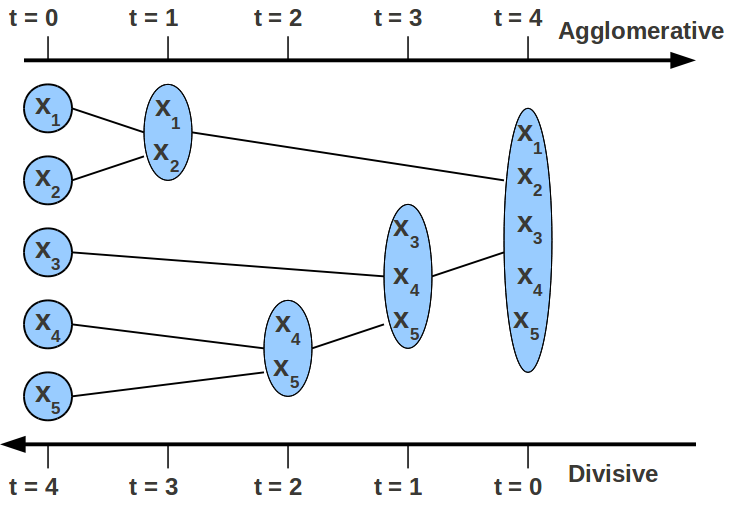
\includegraphics[width=0.6\textwidth]{hierarchical-clustering}
\caption[Etapas del agrupamiento jerárquico]{Etapas del agrupamiento jerárquico \citep{Rai2011}}
\label{fig:hier-clustering}
\end{figure}

\begin{figure}[htbp]
\centering
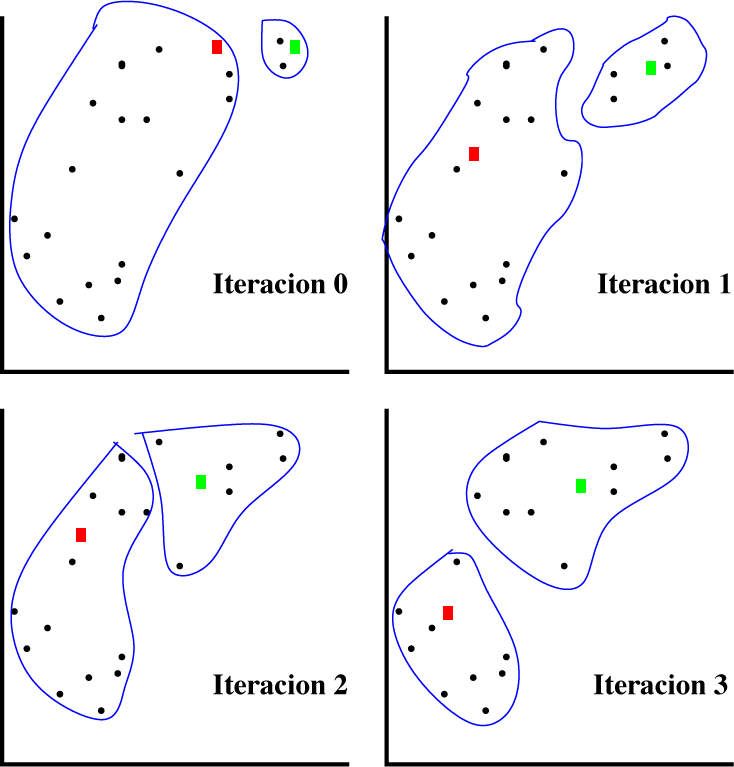
\includegraphics[width=0.6\textwidth]{k-medias}
\caption[Etapas del agrupamiento plano]{Etapas del agrupamiento plano \citep{RuizReina2013}}
\label{fig:k-medias}
\end{figure}

Además, uno de los retos de estos sistemas es cómo representar el conocimiento extraído en el entrenamiento para almacenarlo y usarlo posteriormente.

\section{Clasificadores}

Los clasificadores son programas que dado un documento de entrada, le asocia una categoría o etiqueta. Estos clasificadores han debido ser previamente entrenados mediante una técnica de aprendizaje automático, o bien programados con las reglas apropiadas.

En función del resultado de la clasificación, podemos distinguir dos tipos de clasificadores:
\nopagebreak
\begin{description}
\item[Clasificador binario] En este caso, existen dos posibles categorías a asocias a cada documento. Por ejemplo, un detector de \emph{spam} puede determinar que un mensaje de correo electrónico es spam o no lo es (es \emph{spam} o es \emph{ham}). El resultado puede venir --y es recomendable--, acompañado de un valor de confidencia (probabilidad de haber acertado).
\item[Clasificador múltiple] Aquí el documento puede asignarse a varias categorías, con un valor de confidencia diferente para cada una. Se podría después tener en cuenta solamente la categoría asignada con mayor probabilidad, o bien se infiere que pertenece simultáneamente a las $n$ categorías con mayor probabilidad.
\end{description}


\subsection{Bondad del clasificador (valor-F)}

Para la comparación de sistemas de búsqueda y recuperación de información disponemos de una métrica llamada valor-F\index{valor-F} (\emph{F-score}\index{F-score@\emph{F-score}}, \emph{F-measure}\index{F-measure@\emph{F-measure}} ó \emph{$F_1$ score}\index{F\_1 score@$F_1$ score}) siendo ésta la media armónica de otros dos indicadores \citep[Precisión y exhaustividad]{wikipedia-es}:
\begin{description}
\item[precisión \emph{(precision)}] \index{precisión}\index{precision@\emph{precision}}
Es la fracción de instancias recuperadas que son relevantes.
\begin{eqnarray}
\text{precisión} &=& \frac{|\{\text{relevantes}\}\cap\{\text{recuperados}\}|}{|\{\text{recuperados}\}|}
\end{eqnarray}
\item[exhaustividad \emph{(recall)}] \index{exhaustividad}\index{recall@\emph{recall}}
Es la fracción de instancias relevantes que han sido recuperadas.
\begin{eqnarray}
\text{exhaustividad} &=& \frac{|\{\text{relevantes}\}\cap\{\text{recuperados}\}|}{|\{\text{relevantes}\}|}
\end{eqnarray}
\item[valor-F \emph{(F-score)}] Media armónica de precisión y exhaustividad.
\begin{eqnarray}
F_1 &=& 2\times\frac{\text{precisión}\times\text{exhaustividad}}{\text{precisión}+\text{exhaustividad}}
\end{eqnarray}
\end{description}

Supongamos un clasificador binario:
\begin{itemize}
\item La medida de precisión será el porcentaje de documentos correctamente clasificados dentro del conjunto de prueba.
\item La medida de exhaustividad será el porcentaje de documentos del conjunto de referencia que han sido correctamente clasificados \citep{Perkins2010}.
\end{itemize}
